% Circumscribed Parallelepiped
% Author: Axel Pavillet
\documentclass[tikz,border=10pt]{standalone}
%%%<
\usepackage{verbatim}
\usepackage{amsmath, amssymb}
\usepackage{stmaryrd}
\usepackage{graphicx, subfigure}
\usepackage{color}
\usepackage[all]{xy}
\usepackage{extarrows}
\usepackage{proof}
\usepackage{hyperref}
\usepackage{wrapfig}
\usepackage{multirow}

\begin{document}
	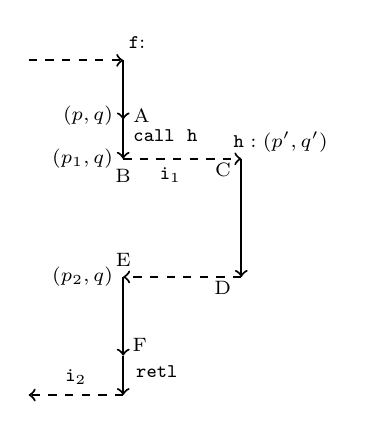
\begin{tikzpicture}[font=\scriptsize, line width=0.75pt]
		\draw[->,dashed] (0.3, 3) -- (1.5, 3);
		\draw[->] (1.5, 3) -- (1.5, 2.25);
		\draw[->] (1.5, 2.25) -- (1.5, 1.75);
		\draw[->,dashed] (1.5, 1.75) -- (3, 1.75);
		\draw[->] (3, 1.75) -- (3, 0.25);
		\draw[->, dashed] (3, 0.25) -- (1.5, 0.25);
		\draw[->] (1.5, 0.25) -- (1.5, -0.75);
		\draw[->] (1.5, -0.75) -- (1.5, -1.25);
		\draw[->,dashed] (1.5, -1.25) -- (0.3, -1.25);
		
		\node[right=5pt, above=0.5pt] (f) at (1.5, 3) {\texttt{f}:};
		\node[right] (A) at (1.5, 2.3) {A};
		\node[right] (call) at (1.5, 2.05) {$\texttt{call} \; \; \texttt{h}$};
		\node[below] (B) at (1.5, 1.75) {B};
		\node[below] (i1) at (2.1, 1.77) {$\texttt{i}_1$};
		\node[below=4pt, left] (C) at (3, 1.75) {C};
		\node[below=4pt, left] (D) at (3, 0.25) {D};
		\node[above] (E) at (1.5, 0.25) {E};
		\node[right=6pt, above=0.5pt] (F) at (1.5, -0.85) {F};
		\node[right=1pt] (retl) at (1.5, -0.95) {\texttt{retl}};
		\node[above=0.01pt] at (0.9, -1.25) {$\texttt{i}_2$};
		
		\node[left] (Apq) at (1.5, 2.3) {$(p, q)$};
		\node[left] (Bpq) at (1.5, 1.75) {$(p_1, q)$};
		\node[above] (Cpq) at (3.5, 1.7) {$\texttt{h} : (p', q')$};
		\node[left] (Epq) at (1.5, 0.25) {$(p_2, q)$};
	\end{tikzpicture}
\end{document}